%\documentclass[10pt,handout]{beamer}
\documentclass[10pt]{beamer}
\usepackage[english]{babel} % Anpassa efter svenska. Ger svensk logga.
\usepackage[utf8]{inputenc} % Anpassa efter linux
\usepackage{graphicx}
\usepackage{../common/beamerthemeUppsala}
%\usecolortheme{UU} % Anpassa efter UU:s frger och logga
%\hypersetup{pdfpagemode=FullScreen} % Adobe Reader ska ppna fullskrm
\setbeamertemplate{itemize items}[circle]

% \usepackage{beamerthemesplit}
\usepackage{amsmath}
\usepackage{amssymb}
% \usepackage{graphics}
% \usepackage{graphicx}
% \usepackage{epsfig}
% \usepackage[latin1]{inputenc}
 \usepackage{color}
% \usepackage{fancybox}
% \usepackage{psfrag}
% \usepackage[english]{babel}
 \setbeamertemplate{footline}{\hfill\insertframenumber/\inserttotalframenumber}


% Read in commands
% Course settings
\newcommand{\currentsemester}{Autumn 2024}

% New commands
\newcommand{\bfm}[1]   {\mbox{\boldmath{${#1}$}}}
\newcommand{\Prob}   {\mbox{\textnormal{P}}}
\newcommand{\uured}[1]{\textcolor{uured}{#1}}

% Eqds
\def\eqd{\,{\buildrel d \over =}\,}

% Math operators
\DeclareMathOperator{\E}{\mathbb{E}}
\DeclareMathOperator{\V}{\mathbb{V}}


%%%%%%%%%%%%%%%%%%%%%%%%%%%%%%%%%%%%%%%%%%%%%%%%%%%%%%%%%%%%%%%%%%

\setlength{\parskip}{3mm}
\title[]{{\color{black}Machine learning -- Block 3}}
\author[]{M{\aa}ns Magnusson\\Department of Statistics, Uppsala University}
\date{\currentsemester}


\begin{document}

\frame{\titlepage
% \thispagestyle{empty}
}



%%%%%%%%%%%%%%%%%%%%%%%%%%%%%%%%%%%%%%%%%%%%%%%%%%%%%%%%%%%%%%%%%%


\section{Practicalities}

\begin{frame}{Evaluation assignment 2}
\begin{itemize}
\item t
\end{itemize}
\end{frame}


\begin{frame}{This week's lecture}
\begin{itemize}
\item Feed-Forward Neural Networks
\item Regularization of Neural Networks
\item Neural Network Optimization
\end{itemize}
\end{frame}


\section{Introduction}
\frame{\sectionpage}

%%%%%%%%%%%%%%%%%%%%%%%%%%%%%%%%%%%%%%%%%%%%%%%%%%%%%%%%%%%%%%%%%%


\frame{\frametitle{The Hype: Computer Vision}

\begin{figure}[h]
\caption{ImageNet performance (Roessler, 2019)}
\centering
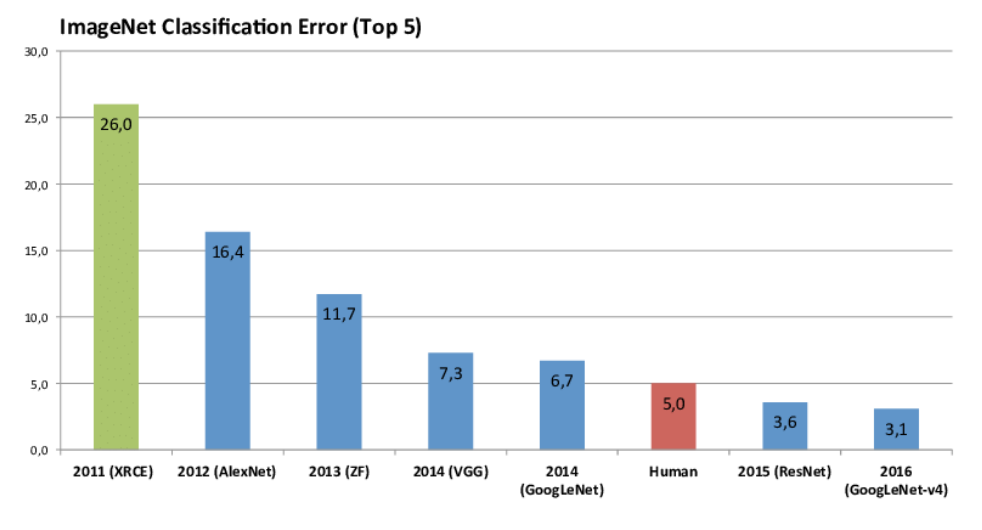
\includegraphics[width=0.8\textwidth]{fig/imageNet.png}
\end{figure}
}


\frame{\frametitle{The Hype: Speech Recognition}

\begin{figure}[h]
\centering
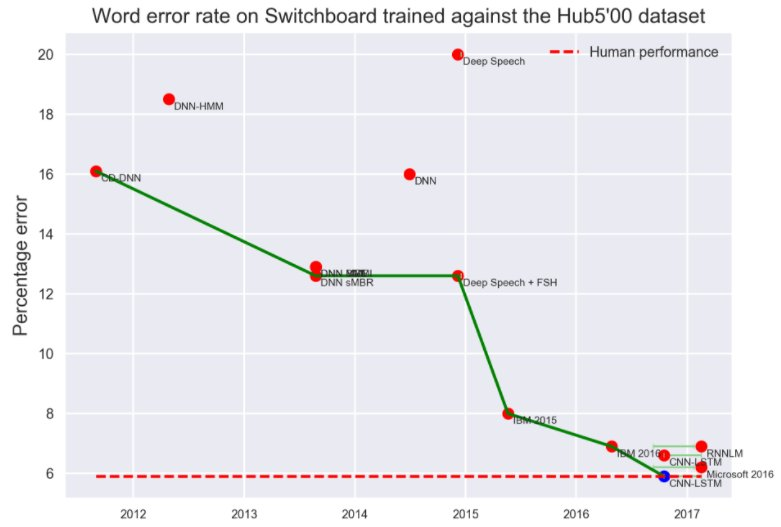
\includegraphics[width=0.8\textwidth]{fig/SP.jpeg}
\caption{Speech recognition performance (source: \url{https://eff.org/ai/metrics})}
\end{figure}
}

\frame{\frametitle{The Hype: Natural Language Processing}

\begin{figure}[h]
\centering
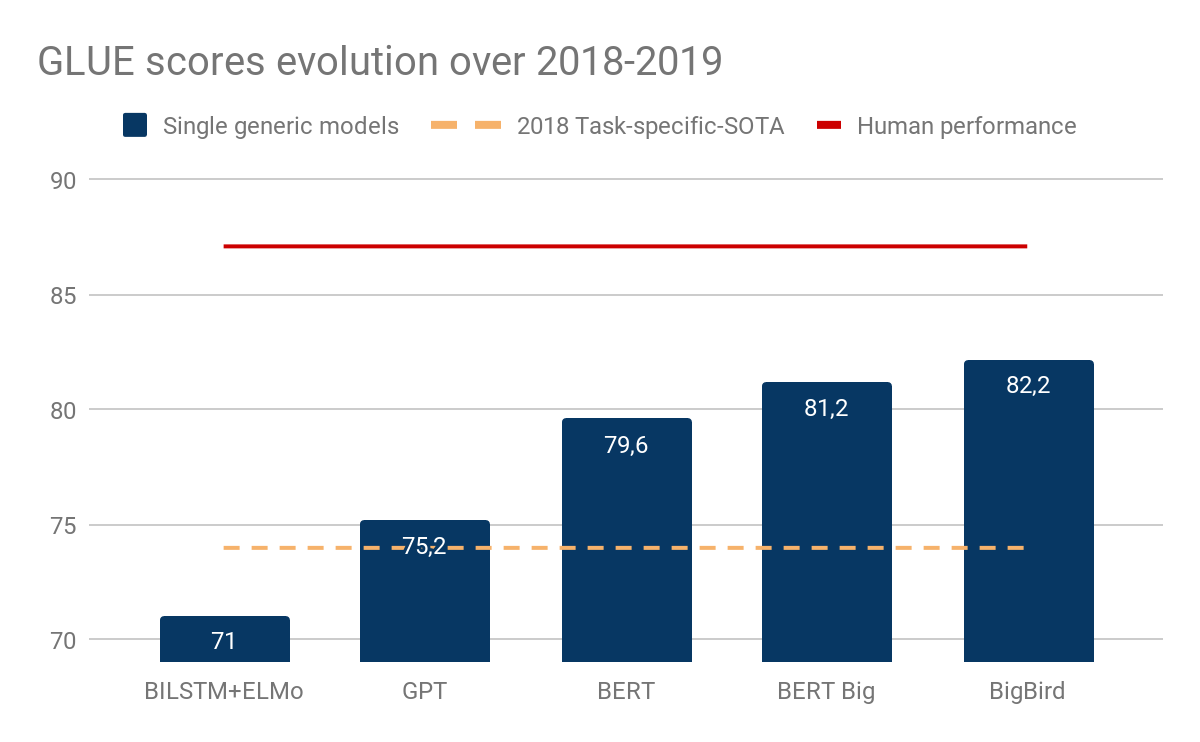
\includegraphics[width=0.8\textwidth]{fig/GLUE.png}
\caption{General Language Understanding (source: \url{https://www.programmersought.com/article/4251948498/})}
\end{figure}

Work is very much ongoing:

\url{https://gluebenchmark.com/leaderboard}


}

\frame{\frametitle{The Hype}

\begin{itemize}
\item Although - Neural Networks is not a silver bullet\pause
\item Remember the {\color{uured} Bayes error}\pause
\item Some times a linear regression (or Random Forest) is enough
\end{itemize}

}


\section{Feed-Forward Neural Networks}
\frame{\sectionpage}

%\subsection{Learning} % And backprop

%\subsection{Hidden Units}

%\subsection{Architecture design}


\frame{\frametitle{The Feed-Forward Network}

\begin{figure}[h]
\centering
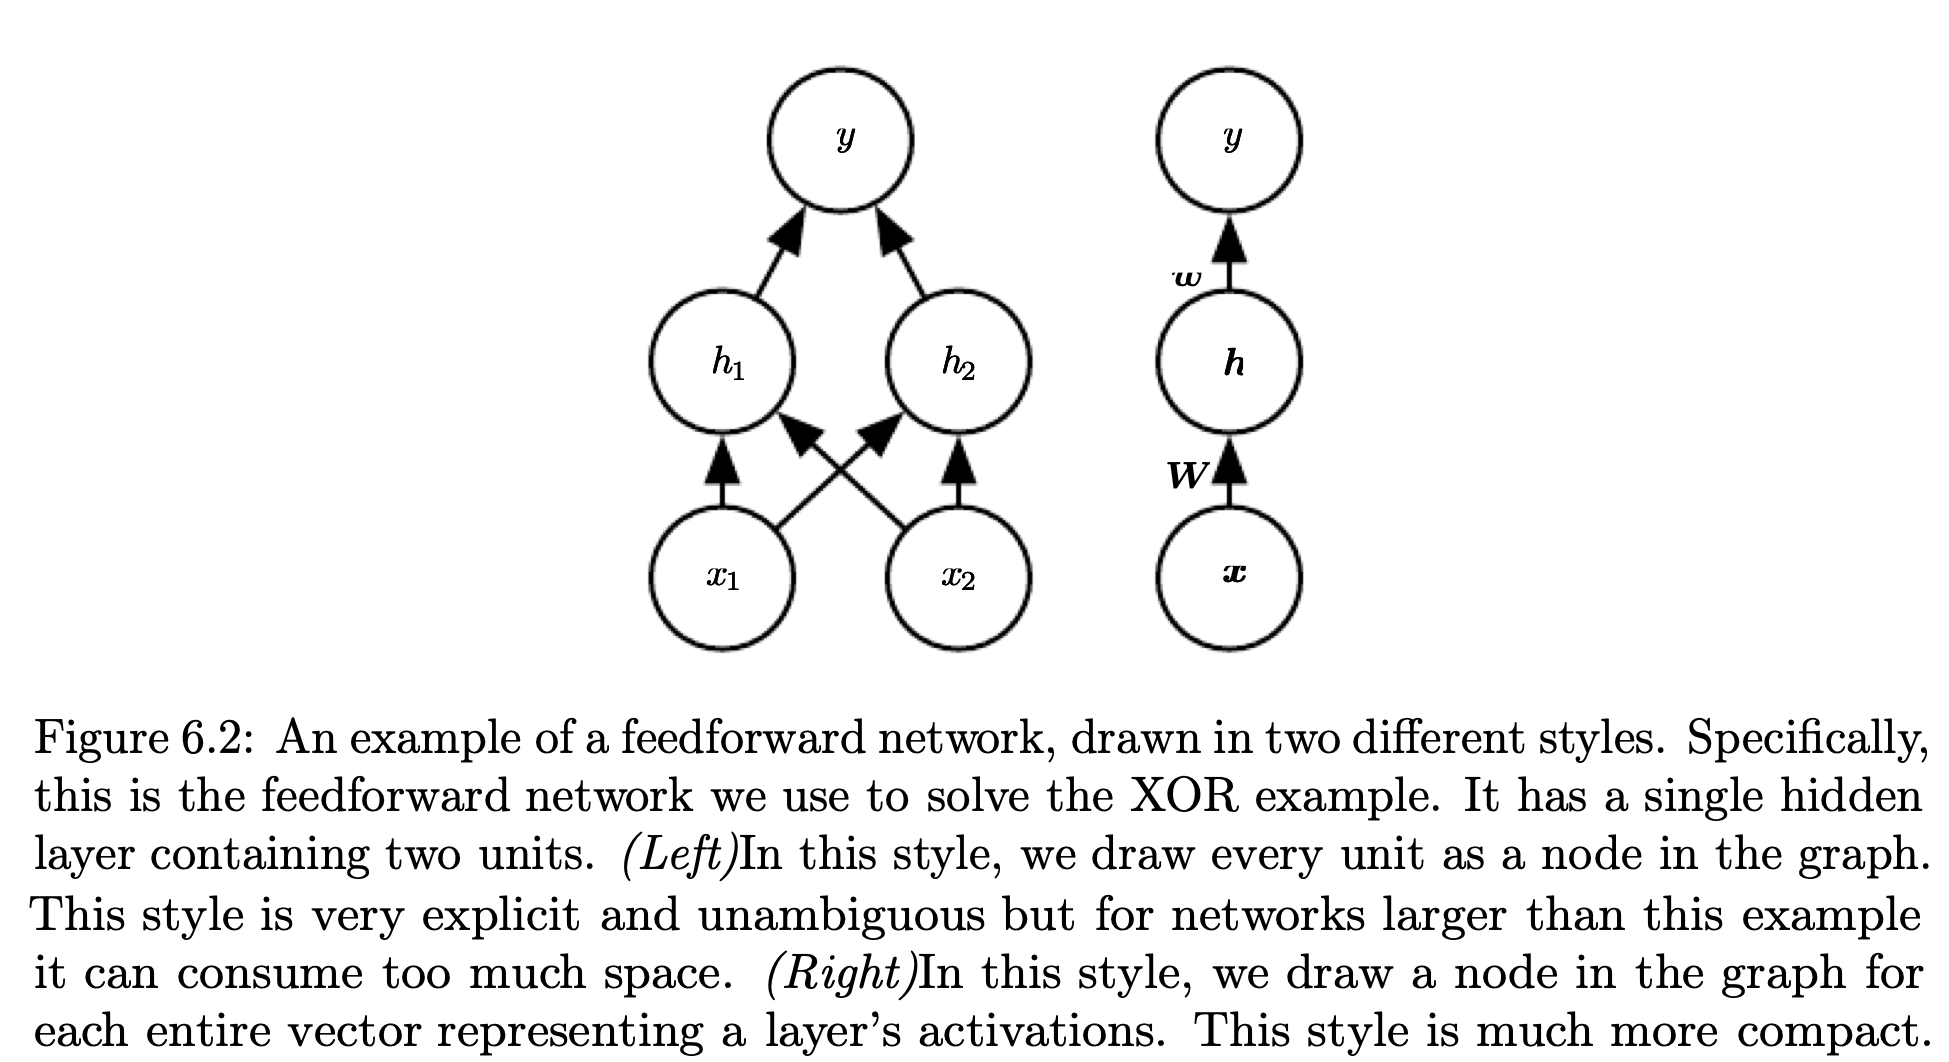
\includegraphics[width=0.8\textwidth]{fig/simple_NN.png}
\caption{A simple feed-forward network (Goodfellow et al, 2017)}
\end{figure}

{\color{uured} Important concepts}:

Layers, neurons, input, output, weights, bias, architecture

}

\frame{\frametitle{Different Architectures for Different Purposes}

\begin{itemize}
\item Different networks for different purposes
\begin{itemize}
\item {\color{uured} Convolutional Neural Networks}: Computer Vision\pause
\item {\color{uured} Recurrent Neural Networks}: Speech Audio (?)\pause
\item {\color{uured} Transformers/Attention}: Textual data
\end{itemize}
\item The Neural Network Zoo: \url{https://www.asimovinstitute.org/neural-network-zoo/}
\end{itemize}

}


\frame{\frametitle{Areas of Use: All fields}

\begin{itemize}
\item Supervised learning
\item Unsupervised learning
\item Reinforcement learning
\end{itemize}

}


\frame{\frametitle{Why and when neural nets?}

\begin{itemize}
\item Learning feature representations
\item Needs a lot of data to learn complex representations
\item Good for sensor data (high-dimensional)\pause
\item When should we not use neural networks?
\end{itemize}

}

\frame{\frametitle{Learning Representations}

\begin{figure}[h]
\centering
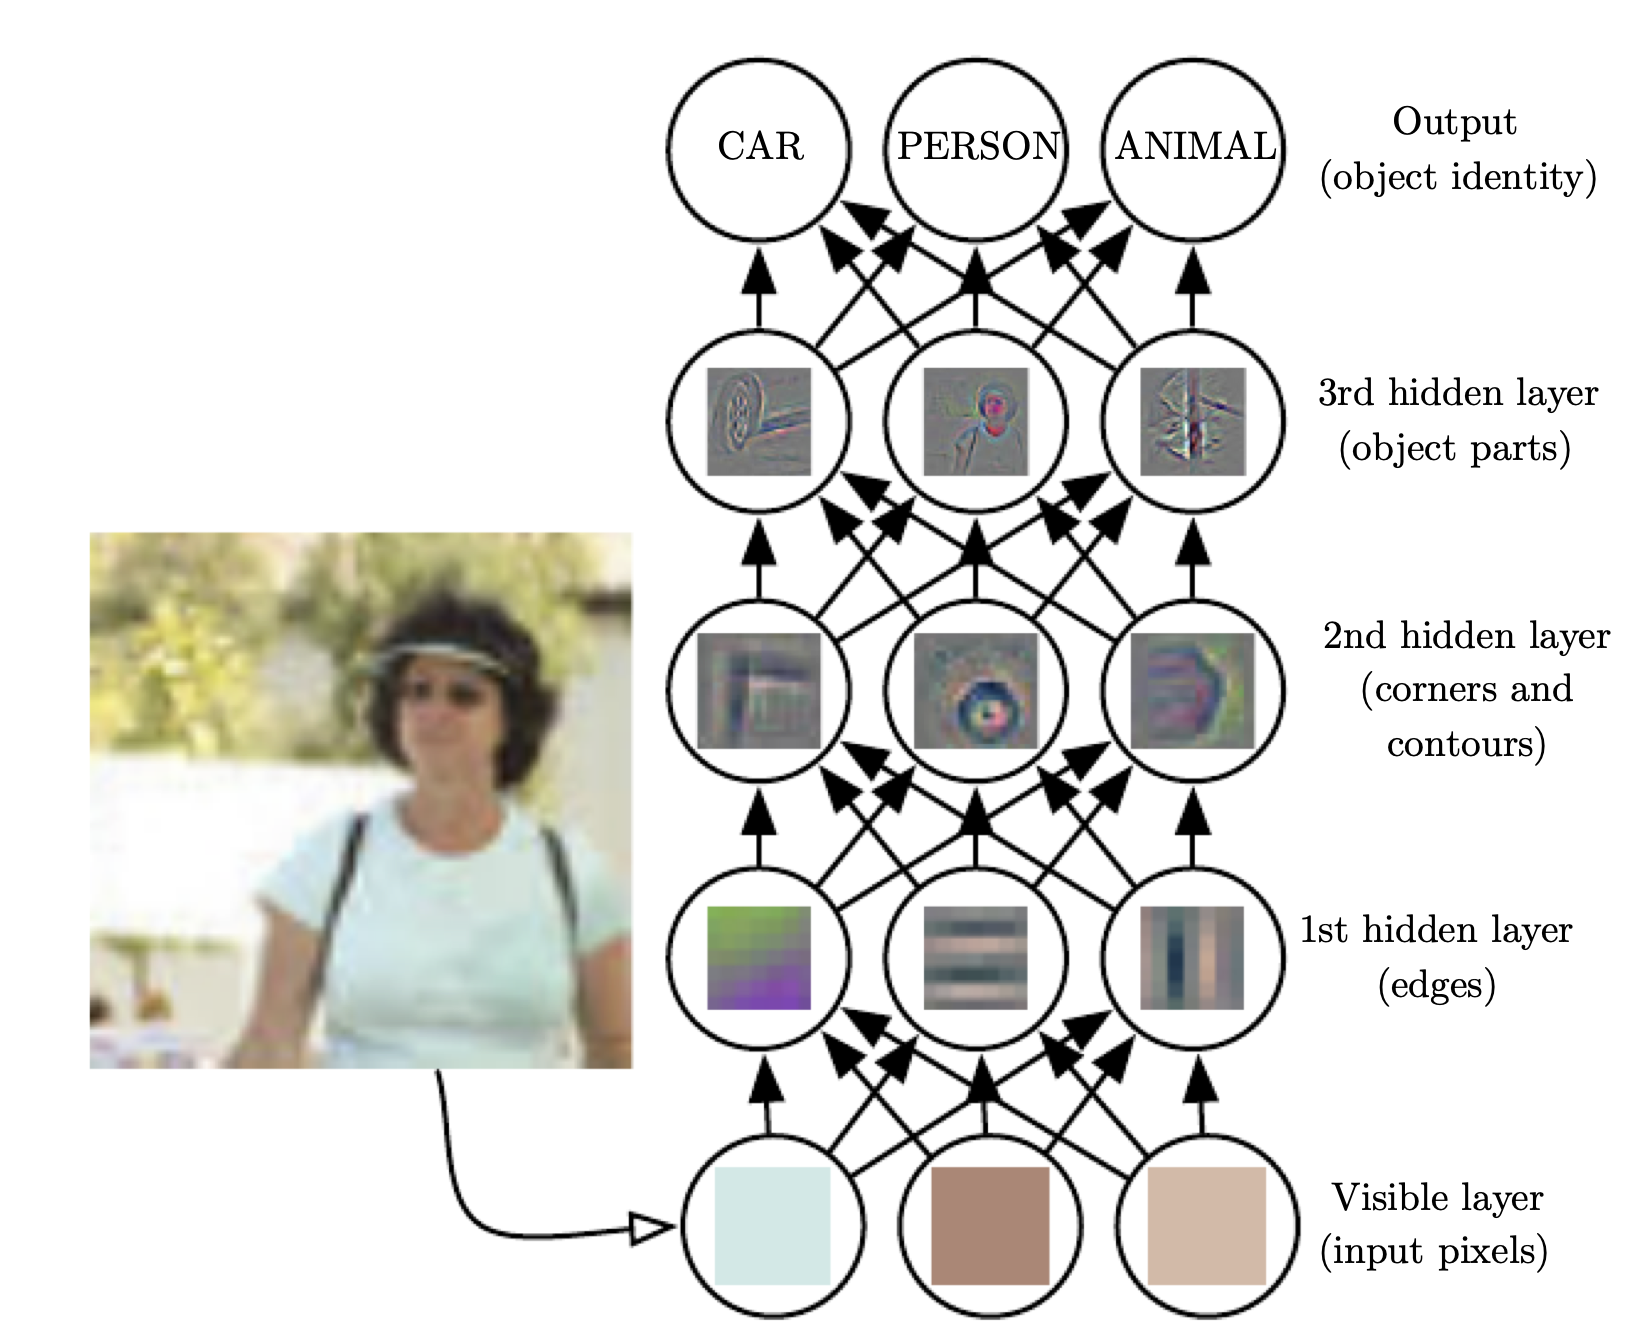
\includegraphics[width=0.8\textwidth]{fig/DL_fig_1_2_representations.png}
\caption{Learning representations can be crucial (Goodfellow et al, 2017, Fig. 1.2)}
\end{figure}

}


\subsection{Feed-Forward Neural Networks}
\frame{\frametitle{The Feed-Forward Network}

\begin{figure}[h]
\centering
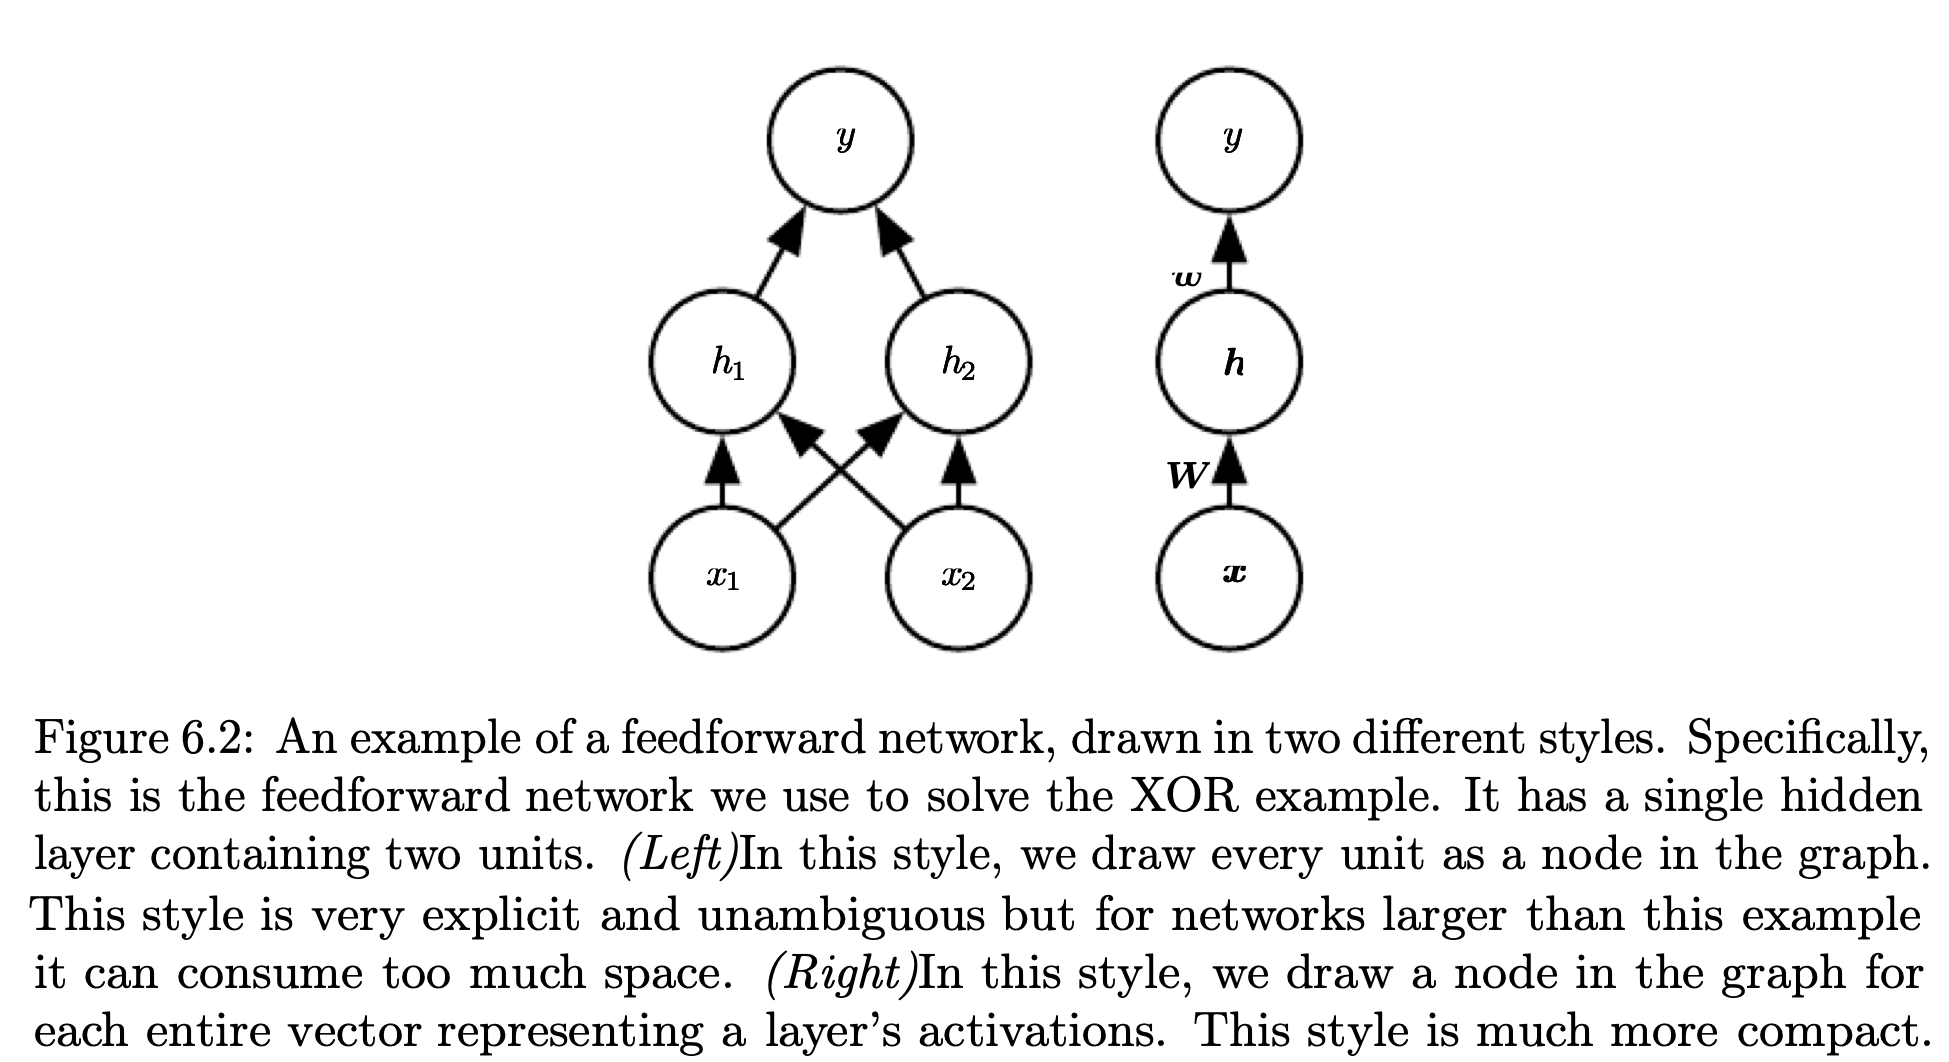
\includegraphics[width=0.8\textwidth]{fig/simple_NN.png}
\caption{A simple feed-forward network (Goodfellow et al, 2017, Fig. 6.2)}
\end{figure}

In mathematical notation:
\[
y_i = \mathbf{w}^T g(\mathbf{W}^T\mathbf{x}_i + \mathbf{b}_1) + \mathbf{b}_2
\]

}

\frame{\frametitle{The Feed-Forward Network}

\[
y_i = \mathbf{w}^T g(\mathbf{W}^T\mathbf{x}_i + \mathbf{b}_1) + \mathbf{b}_2
\]

\begin{equation*}
W =
\begin{pmatrix}
1 & 1 \\
1 & 1 \\
\end{pmatrix}
\,,w =
\begin{pmatrix}
1 \\
-2 \\
\end{pmatrix}\,,
b_1 =
\begin{pmatrix}
1 \\
-1 \\
\end{pmatrix}\,,
b_2 =
\begin{pmatrix}
0 \\
\end{pmatrix}
\end{equation*}

\begin{equation*}
g(z) = ReLU(z) = \max(0,z)\,,
x_i =
\begin{pmatrix}
0 \\
0 \\
\end{pmatrix}\,,
\end{equation*}

\[
y_i = \begin{pmatrix}
1 \\
-2 \\
\end{pmatrix}^T g(\begin{pmatrix}
0 \\
0 \\
\end{pmatrix} +
\begin{pmatrix}
1 \\
-1 \\
\end{pmatrix}
) + \begin{pmatrix}
0 \\
\end{pmatrix}
\]
\[
y_i = \begin{pmatrix}
1 \\
-2 \\
\end{pmatrix}^T \begin{pmatrix}
1 \\
0 \\
\end{pmatrix} + \begin{pmatrix}
0 \\
\end{pmatrix} = 1
\]

}



\frame{\frametitle{The Feed-Forward Network}

A feed-forward network for one observation ($x_i$).

\begin{align*}
\underbrace{\mathbf{h}_1}_{1 \times k_1} &= g_1(\underbrace{\mathbf{x}^{T}}_{1 \times p}\underbrace{\mathbf{W}_1}_{p \times k_1} + \underbrace{\mathbf{b}_1}_{1 \times k_1}) \\
& \vdots \\
\underbrace{\mathbf{h}_l}_{1 \times k_l}  &=  g_l(\underbrace{\mathbf{h}_{l-1}^{T}}_{1 \times k_{l-1}}\underbrace{\mathbf{W}_l}_{k_{l-1} \times k_l} + \underbrace{\mathbf{b}_l}_{1 \times k_l}) \\
& \vdots \\
\underbrace{\hat{\mathbf{y}}}_{1 \times m} &= g_{L}(\underbrace{\mathbf{h}^{T}_{{L-1}}}_{1 \times k_{l-1}}\underbrace{\mathbf{W}_{L}}_{k_{l-1} \times m} + \underbrace{\mathbf{b}_{L}}_{1 \times m})
\end{align*}

\[
\hat{y} = f_L(f_{L-1}(...f_1(x)...))
\]

% TODO Fix mathbf

}


\frame{\frametitle{Activation functions ($g_l$)}

\begin{itemize}
\item Sometimes use notation $\sigma$ as in $\sigma(W h + b)$\pause
\item Historically $g(z)$ has been the sigmoid or or hyperbolic tangent (tanh)
\[
g_\text{sigmoid}(z)={\frac {e^{z}}{e^{z}+1}}={\frac {1}{1+e^{-z}}}
\]
\[
g_\text{tanh}(z)={\frac {\sinh z}{\cosh z}}={\frac {e^{2z}-1}{e^{2z}+1}}
\]
\pause
\item Now, usually variants of Rectified linear unit (ReLU)
\[
g_\text{ReLU}(z)=\max({0,z})
\]
\begin{itemize}
\item Easier to estimate with SGD
\item Easier for deep models
\end{itemize}
\item Last activation is the output function $g_L$, usually a softmax (if classification)
\[
f(z_i)={\frac {e^{z_i}}{\sum _{j=1}^{J}e^{z_{j}}}}
\]
\end{itemize}

}



\frame{\frametitle{Activation functions ($g_l$)}

\begin{figure}[h]
\centering
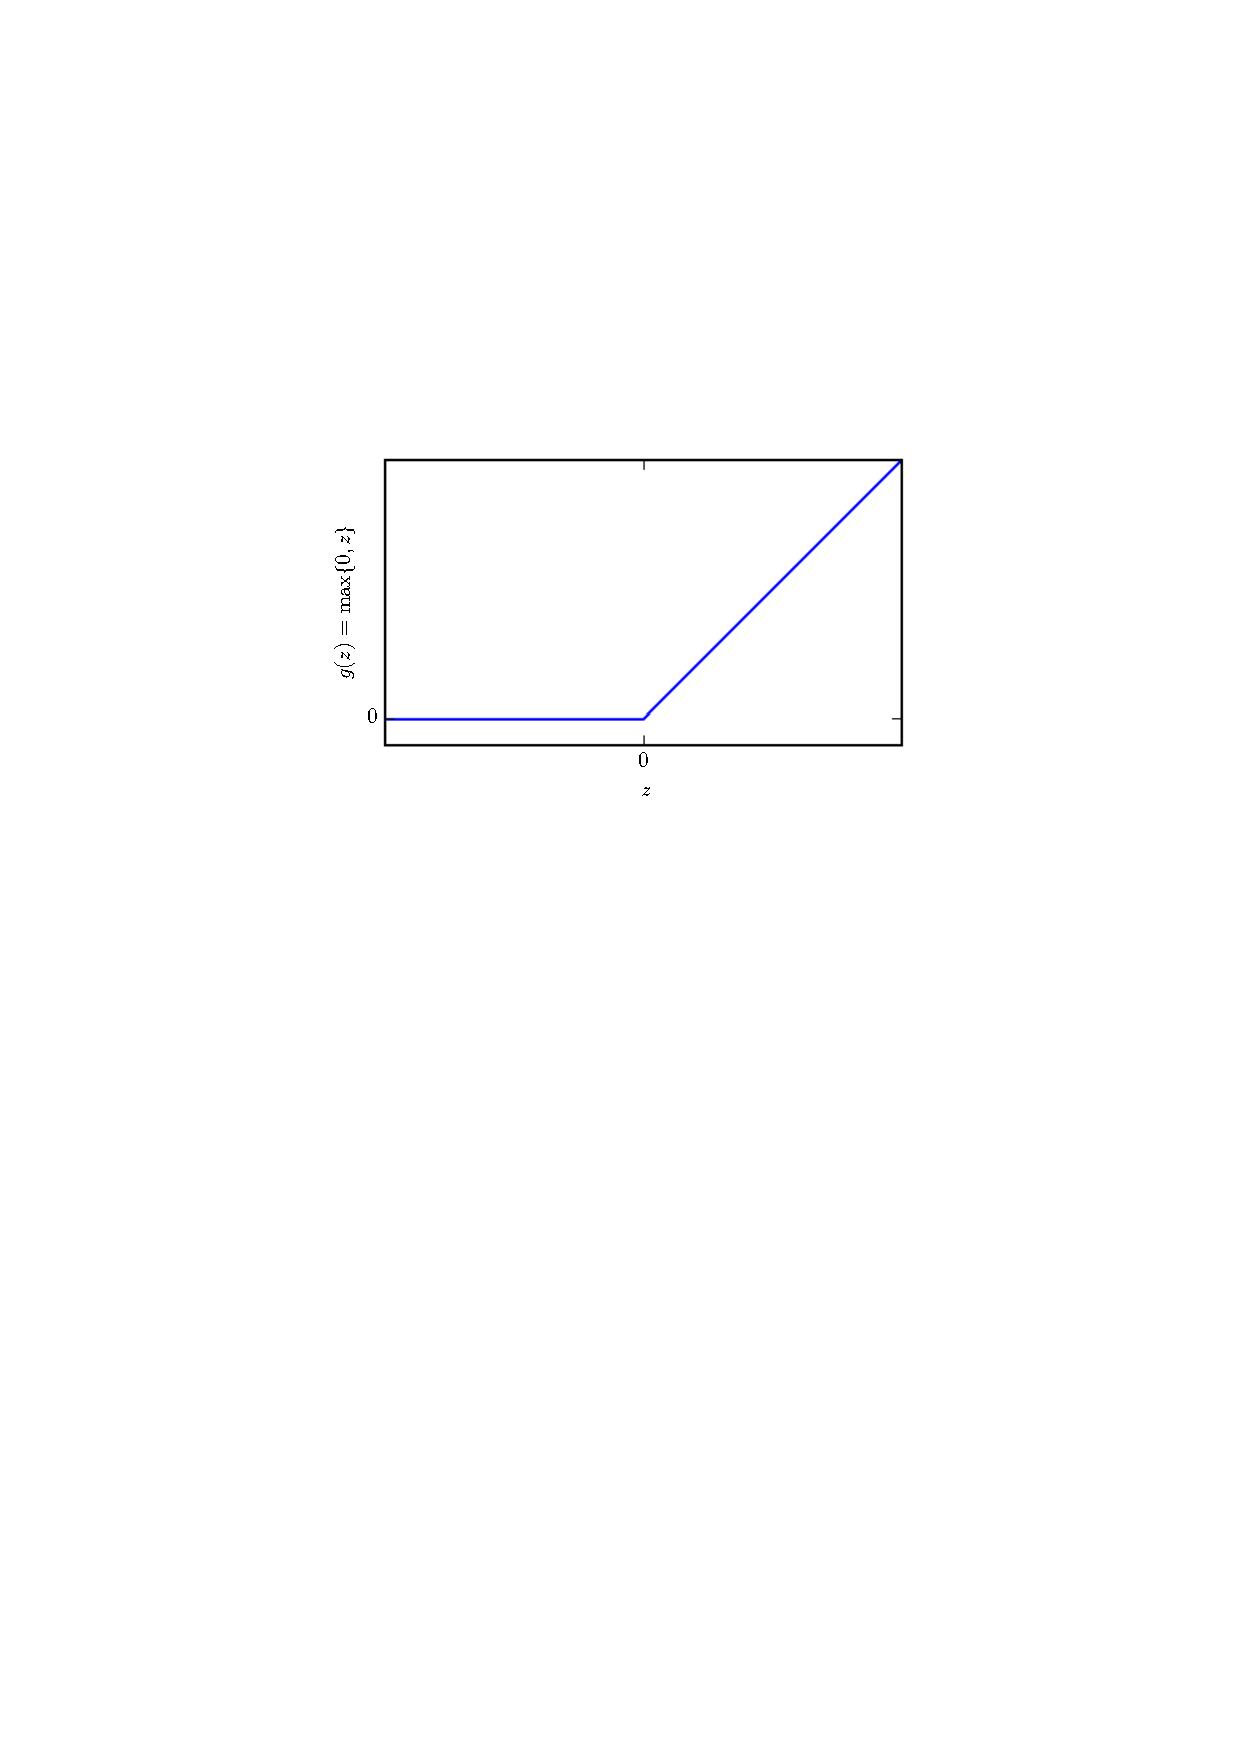
\includegraphics[width=0.6\textwidth]{fig/ReLu.pdf}
\caption{Rectified Linear Unit (Goodfellow et al, 2017, Fig. 6.3)}
\end{figure}

}


\frame{\frametitle{Universal Approximation Theorem}

"A feed-forward neural network with a linear output layer and at least one hidden layer with any 'squashing' activation function can approximate any Borel measurable function from one finite-dimensional space to another with any desired non-zero amount of error, provided that the network is given enough hidden units." (Goodfellow et al. 2017, p. 198)

\begin{itemize}
\item Also holds for ReLU
\item No garantuee we can learn the network
\item No garantuee that it will generalize
\item No indication of how large the network need to be
\end{itemize}

}

\subsection{Hyper-parameters}

\frame{\frametitle{Hyper-parameters in feed-forward networks}

\begin{itemize}
\item The number of layers
\item The number of neurons
\item Activation functions
\item The type of layers (CNN, MaxPooling, Multi-head attention)
\end{itemize}

}

\frame{\frametitle{How to choose parameters}

\begin{itemize}
\item Trial and error on validation sets
\item Art rather than science
\item Specialized approaches (Bayesian Optimization)\pause
\item Grid search (combinatorical explosion)
\begin{itemize}
\item Really bad with many parameters with less effects
\item If we have 5 irrelevant parameters we try 3 values for: 125 training per relevant run
\item Instead use...\pause
\end{itemize}
\item Random search
\end{itemize}

}

\frame{\frametitle{Grid search vs. Random Search}

\begin{figure}[h]
\centering
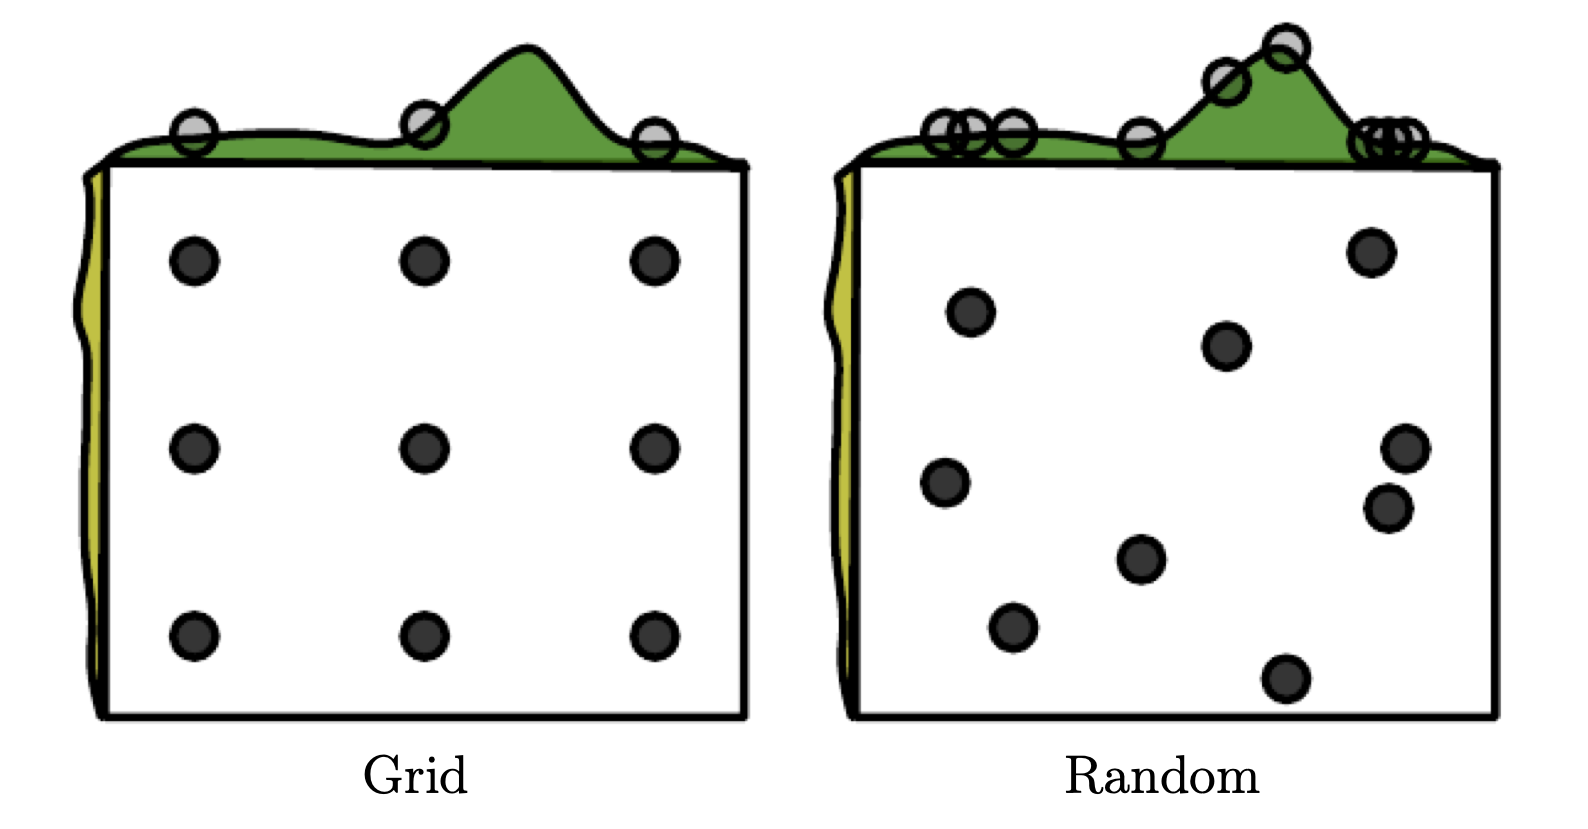
\includegraphics[width=0.6\textwidth]{fig/random_search.png}
\caption{Grid search and random search (Goodfellow et al, 2017, Fig. 11.2)}
\end{figure}

}




\section{Regularization}
\frame{\sectionpage}

\frame{\frametitle{Regularization of Neural Networks}

\begin{itemize}
\item Reduce traing error but improve test/validation error\pause
\item Neural Networks are extremely flexible / high model capacity\pause
\item Regularization is crucial for good generalizability
\end{itemize}

}

\subsection{Norm penalty}
% 7.1

\frame{\frametitle{Weight decay / Norm penalty}

\begin{itemize}
\item Let
\[
\tilde{J}(W,b) = J(W,b) + \alpha \Omega(W)\,,
\]
where $J(W,b)$ is the cost function and $\alpha \Omega(W)$ is the penalty for the weight matrices.
\item $\alpha$ is the strength of the penalty.
\end{itemize}

}

\frame{\frametitle{Weight decay / Norm penalty}

\begin{itemize}
\item Let
\[
\Omega_1 (W) = \sum_i \sum_j |w|_{i,j}\,,
\]
and
\[
\Omega_2 (W) = \sum_i \sum_j w^2_{i,j}\,,
\]
be the $L_1$ and $L_2$ regularization respectively.
\item We can then get the cost function
\[
\tilde{J}(W,b) = J(W,b) + \sum_l \alpha_l \Omega_2(W_l)\,,
\]
\end{itemize}

}


\frame{\frametitle{Weight decay / Norm penalty}

\begin{itemize}
\item Lets define the cost function as
\begin{align*}
\tilde{J}(w) &= J(w) + \alpha \Omega_2(w)\\
             &= J(w) + \alpha w^T w
\end{align*}
\item Then the gradient update becomes
\begin{align*}
\nabla_w \tilde{J}(w) &= \nabla_w J(w) + 2\alpha w
\end{align*}
\item To update our weights with gradient descent
\begin{align*}
w \leftarrow & w - \epsilon( \nabla_w J(w) + 2\alpha w)\\
w \leftarrow & (1 - 2\alpha \epsilon)w - \epsilon \nabla_w J(w)\\
\end{align*}
\end{itemize}

}


\frame{\frametitle{Weight decay / Norm penalty}

\begin{figure}[h]
\centering
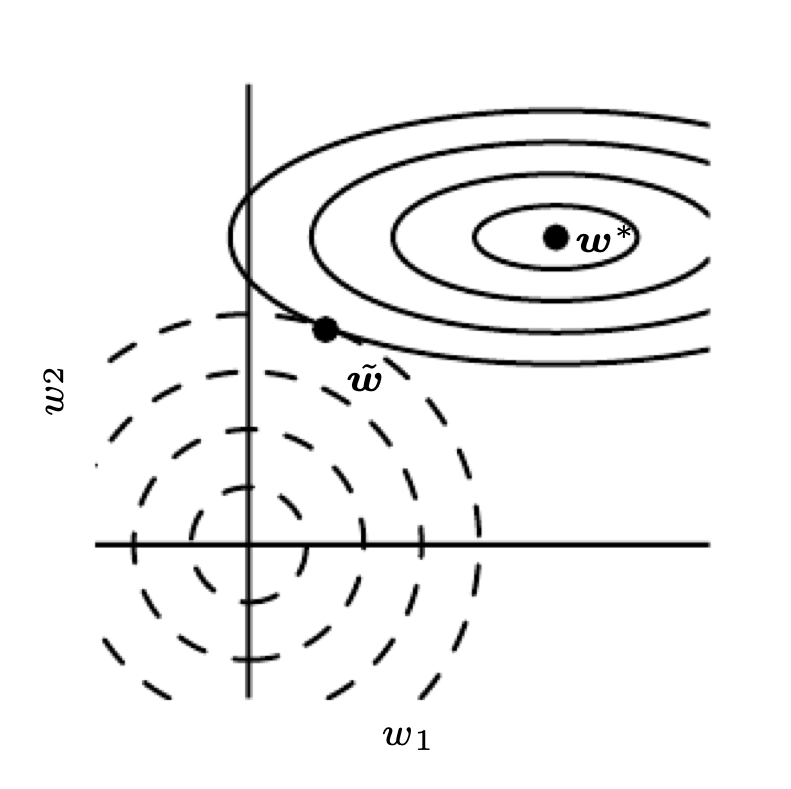
\includegraphics[width=0.6\textwidth]{fig/L2.png}
\caption{$L_2$ regularization (Goodfellow et al, 2017, Fig. 7.1)}
\end{figure}

}


\subsection{Data augmentation}
% 7.4

\frame{\frametitle{Dataset augmentation}

\begin{figure}[h]
\centering
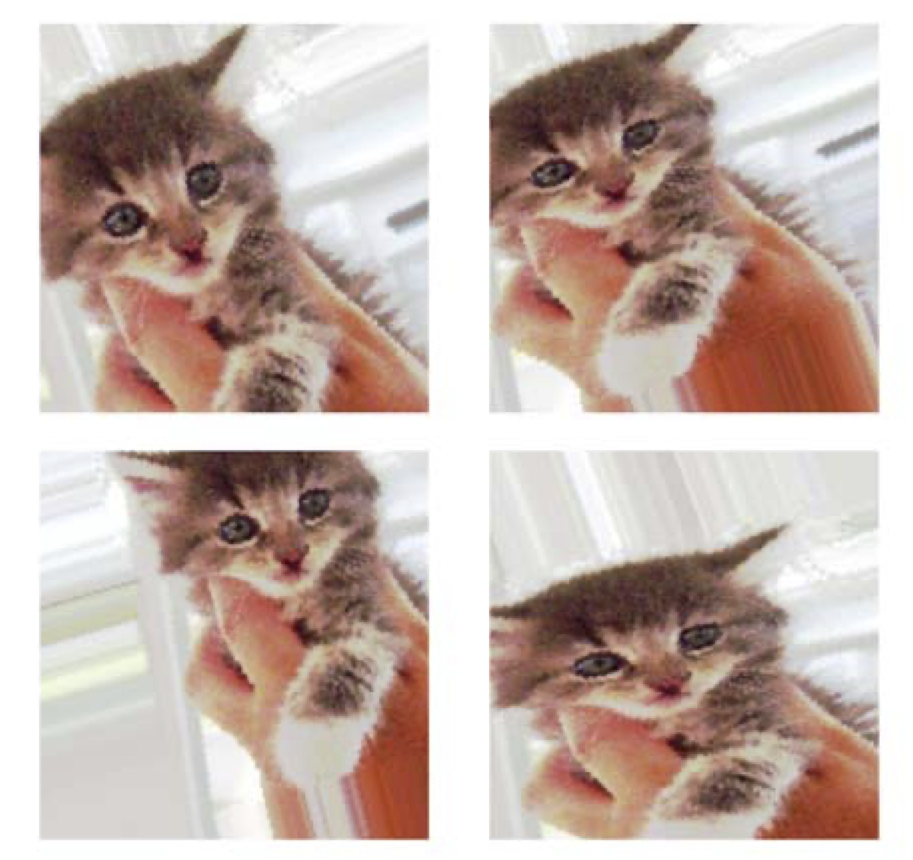
\includegraphics[width=0.5\textwidth]{fig/DLR_fig_5_10_data_augmentation.png}
\caption{Data Augmentation (Chollet and Allair, 2018, Fig 5.10)}
\end{figure}
\begin{itemize}
\item "Modify" data or inject noise
\item Common in Convolutional neural networks
\end{itemize}
}

\subsection{Multi-Task Learning}
% 7.7

\frame{\frametitle{Multi-Task Learning}

\begin{figure}[h]
\centering
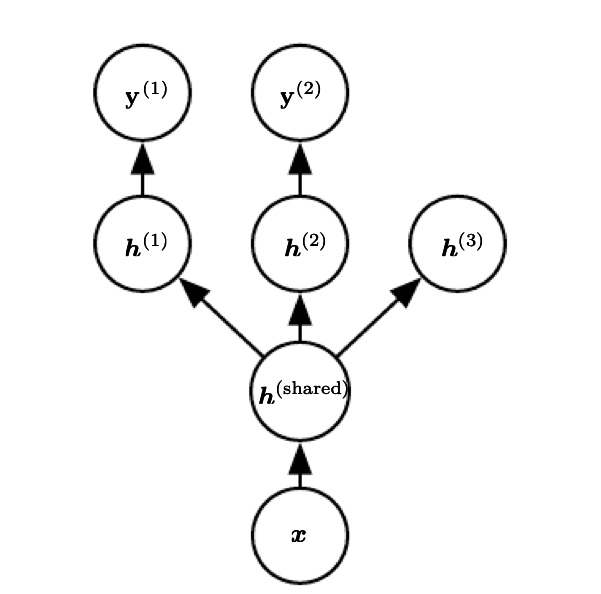
\includegraphics[width=0.5\textwidth]{fig/DL_7_2.png}
\caption{Multi-task learning (Goodfellow et al., 2017, Fig 7.2)}
\end{figure}
\begin{itemize}
\item Common in Large Language Models (Transformers)
\end{itemize}
}

\subsection{Early Stopping}
% 7.8


\frame{\frametitle{Early Stopping}

\begin{itemize}
\item Stop optimization early based on validation error
\item Rerun to that number of epochs (hyperparameter)
\item Can be shown to be quivalent (under strict assumptions) to $L_2$ regularization
\end{itemize}

\begin{figure}[h]
\centering
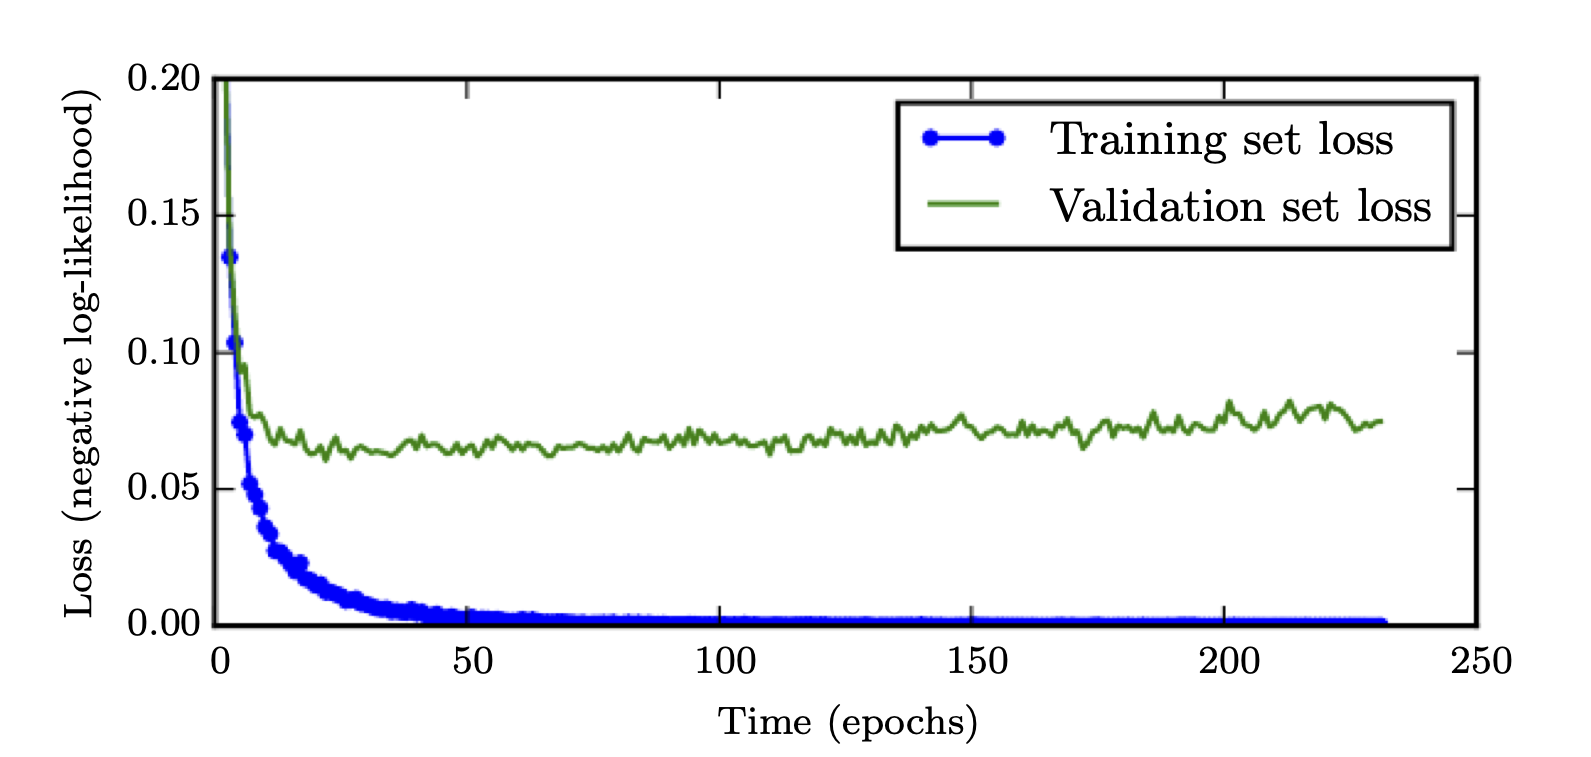
\includegraphics[width=0.8\textwidth]{fig/early_stopping.png}
\caption{Early Stopping (Goodfellow et al, 2017, Fig. 7.3)}
\end{figure}
}

\frame{\frametitle{Early Stopping}

\begin{figure}[h]
\centering
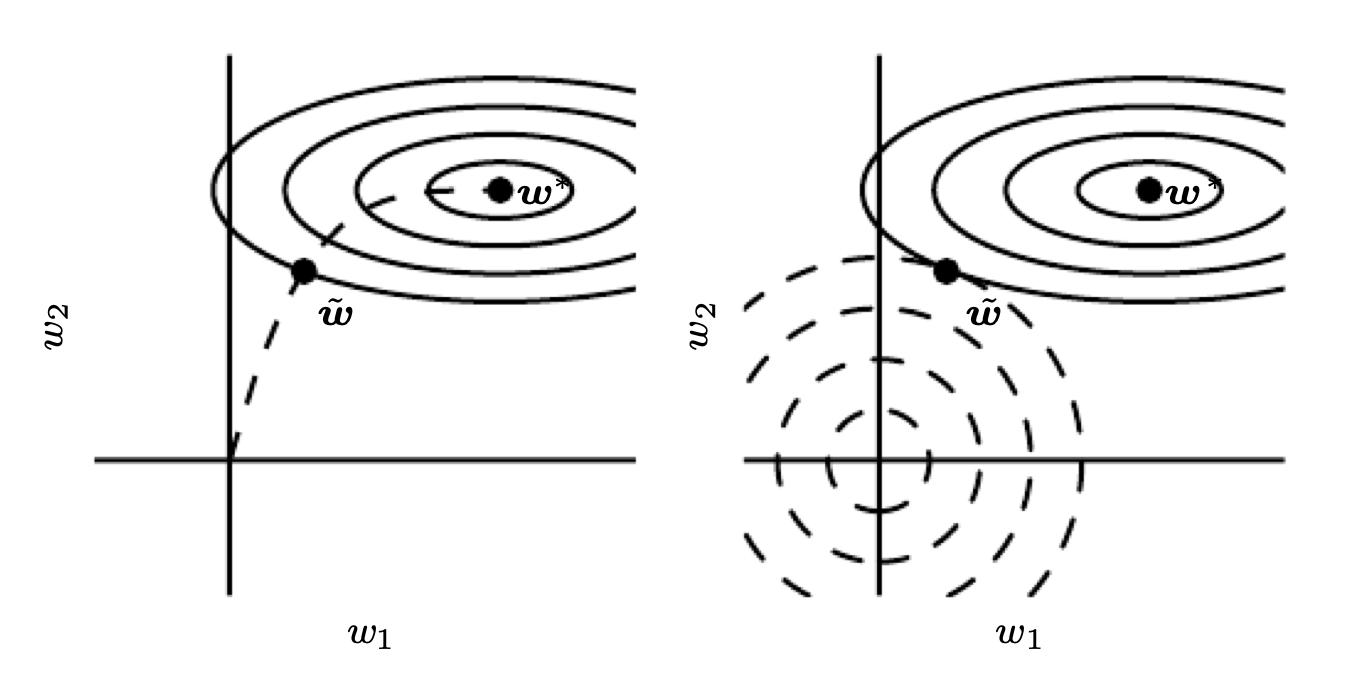
\includegraphics[width=0.8\textwidth]{fig/early_stopping_L2.png}
\caption{Early Stopping (Goodfellow et al, 2017, Fig. 7.4)}
\end{figure}
}

\subsection{Drop-out}
% 7.12

\frame{\frametitle{Dropout}

\begin{itemize}
\item In each iteration:
\begin{itemize}
\item Sample an indicator $I_i$ for each node $i$
\item Set the value $h_i$ to 0 with probability $p$
\end{itemize}
\item The dropout probability is typically 0.8 for input nodes and 0.5 for hidden nodes
\item Forces the network to
\begin{itemize}
\item not rely on individual nodes
\item spread out the weights over more nodes
\end{itemize}
\item Can be seen as an ensamble method
\end{itemize}
}


\frame{\frametitle{Dropout}


\begin{figure}[h]
\centering
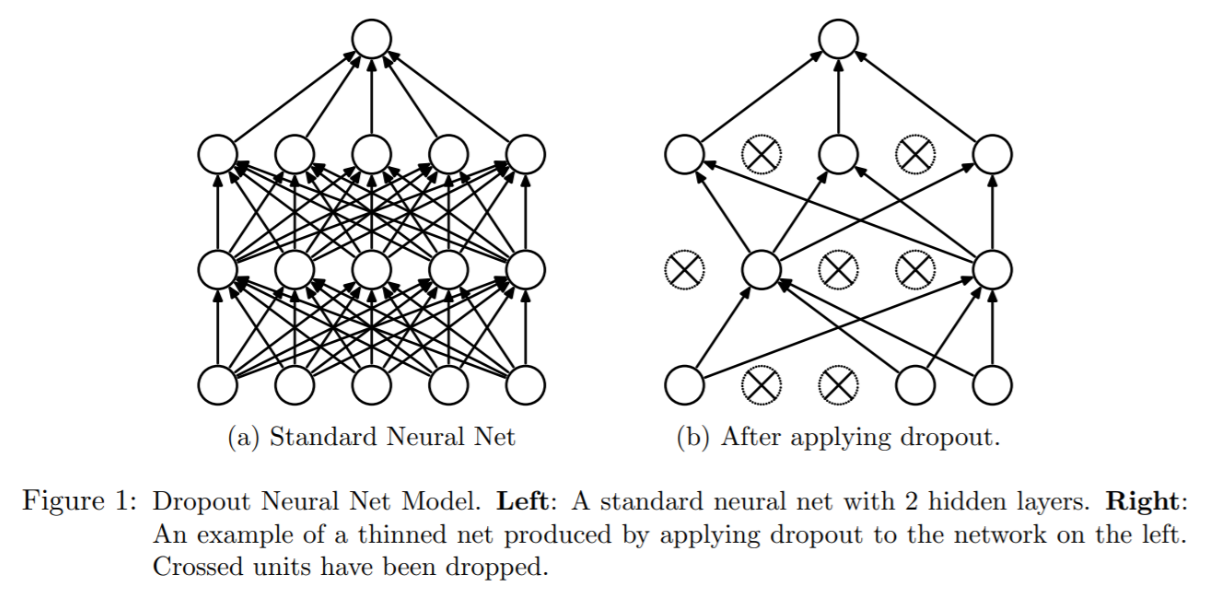
\includegraphics[width=1\textwidth]{fig/dropout.png}
\caption{Dropout (Srivastava et al, 2014)}
\end{figure}

}


\frame{\frametitle{But...}

The best regularizer is... \pause \uured{to get more data}.

}

\section{Optimization of Neural Networks}
\frame{\sectionpage}

\frame{\frametitle{Neural Network Learning}

\begin{itemize}
\item Usually, a lot of data and many parameters ($\theta = (W, b)$)\pause
\item We usually minimize our training cost function
\[
J(\theta) = \sum_i^N L(\text{NN}(x_i),y_i) + \Omega(\theta)\,,
\]
where $L$ is the observation level loss, $\text{NN}()$ is our neural network and $\Omega$ is the regularization term. \pause
\item \uured{Learning Target}: Find $\hat{\theta}$ that minimize the \uured{generalization} error \pause
\end{itemize}

}


\frame{\frametitle{Optimization of Neural Networks}

\begin{itemize}
\item Stochastic Gradient Descent methods
\[
\theta_t = \theta_{t-1} - \eta_t \hat{\nabla} J(\theta_{t-1})
\]
\item In practice, better optimizers are used:
\begin{itemize}
\item Adam
\item RMSprop
\end{itemize}\pause
\item To compute gradients ($\hat{\nabla} J(\theta_{t-1})$):
\begin{itemize}
\item \uured{Backpropagation} algorithm (chain-rule for derivatives)
\end{itemize}
\end{itemize}

% Double check that backprop is introduced before/elaborate more in backprop

}

% TODO: Add
%\subsection{Ill-Conditioning}
% 8.2.1

\subsection{Local minima}

\frame{\frametitle{Problems: Local Minima}
% 8.2.2
\begin{itemize}
\item Neural Networks cost function $J(\theta)$ are (usually) \uured{not a convex} function
\item We can have local minima
\item \uured{When will this be a problem?}\pause
\item A problem if local optima has a \uured{high cost}\pause
\item \uured{Good thing:} This is probably not the situation!\pause
\item Many practitioners believe this is a problem\pause
\item \uured{Diagnosis:} Plot the gradient norm, $\mathbf{g}^T \mathbf{g}$, where $\mathbf{g} = \hat{\nabla} J(\theta)$ \pause
\end{itemize}

}



\subsection{Plateaus and Saddle Points}
% 8.2.3

\frame{\frametitle{Problems: Plateaus and Saddle Points}
% 8.2.3
\begin{itemize}
\item Another problem is \uured{saddle points}
\begin{figure}[h]
\centering
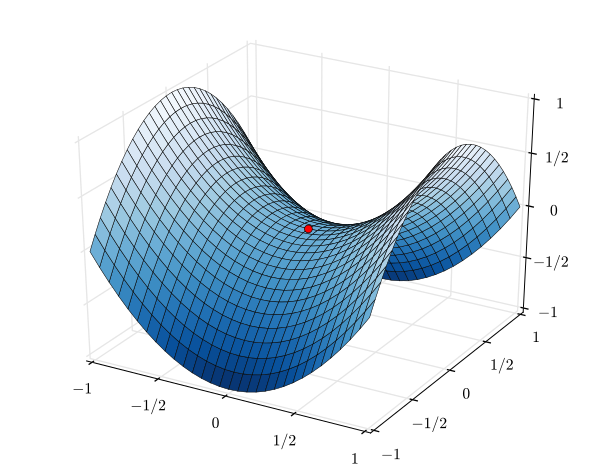
\includegraphics[width=0.8\textwidth]{fig/saddle_point.png}
\caption{Saddle point for $z = x^2 - y^2$ (Wikipedia)}
\end{figure}
\item \uured{What is the gradient in a saddle point?} \pause

\end{itemize}

}

\frame{\frametitle{Problems: Plateaus and Saddle Points}
% 8.2.3
\begin{itemize}
\item In a saddle point the Hessian is \uured{indefinite}, both positive and negative eigen values \pause
\item A local minimum: Hessian is \uured{positive definite}, only positive eigen values \pause
\item In random functions of \uured{high dimension}: \uured{most points are saddle points}
\item \uured{Intuition}: In random functions the sign of the eigen values of the Hessian is random \pause
\item In random functions: eigen values become more positive in regions of lower cost. I.e. local minima more probable in low cost regions. Saddle points more common in high-cost regions\pause
\item The problem of saddle points:
\begin{itemize}
\item Probably a reason why second order methds (using the Hessian) has not succeed
\item Empirically, (stochastic) gradient descent seem to escape saddle points
\end{itemize}
\end{itemize}

}


\subsection{Cliffs, exploding and vanishing gradients}
% 8.2.4-8.2.5
% Copy image 8.2.3

\frame{\frametitle{Problems: Cliffs}
% 8.2.3
\begin{itemize}
\item Another problem is \uured{"cliffs"} or large changes in gradients
\begin{figure}[h]
\centering
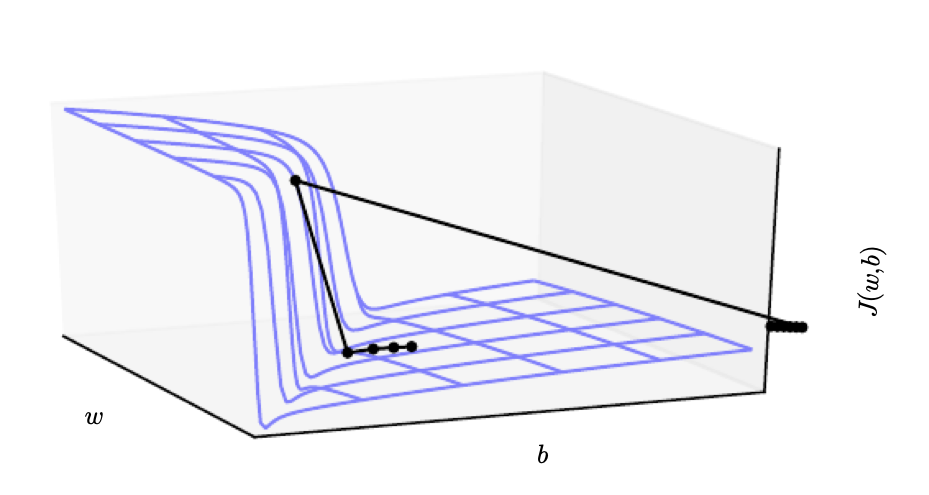
\includegraphics[width=0.8\textwidth]{fig/Dl_8_3.png}
\caption{Cliff (Goodfellow et al., 2017, Fig. 8.3)}
\end{figure}
\item Can undo many iterative steps
\item Common in \uured{Recurrent neural networks}
\item \uured{Mitigation:} Gradient clipping
\end{itemize}
}

\frame{\frametitle{Problems: Explodig and vanishing gradients}
% 8.2.3
\begin{itemize}
\item In deep neural networks, gradients can \uured{vanish or explode}
\item As an example: We want to compute the gradient for a situation where thw weights are multiplied $t$ times. Then using eigendecomposition
\[
W^t = V \text{diag}(\lambda)^t V^T
\]
\item The gradient is scaled wrt $\text{diag}(\lambda)^t$\pause
\item Cliffs is an example of gradient explosion
\item \uured{Mitigation for graident explosion:} Gradient clipping\pause
\item Common problem in \uured{Recurrent neural networks}
\end{itemize}
}

%\subsection{Inexact and difficult gradients}
% 8.2.6
% TODO



\subsection{Parameter initialization}
% 8.4

\frame{\frametitle{Initial values}
\begin{itemize}
\item We need to have \uured{starting values} for gradient descent\pause
\item Initialization can be seen as a hyperparameter\pause
\item Bad initial values might
\begin{itemize}
\item Bad convergence (local optimum)
\item Numerical problems
\end{itemize}\pause
\item We want to \uured{break symmetry} between layers
\begin{itemize}
\item Otherwise the same units will be updated in the same way (deterministically)
\end{itemize}
\pause
\item Good practice
\begin{itemize}
\item Initialize values randomly close to zero (uniform or normal)
\end{itemize}
\end{itemize}

}

% TODO
%\frame{\frametitle{Batch normalization}
%
%\begin{itemize}
%\item A way to simplify the optimization
%\end{itemize}
% TODO: Fix this part - add information here on batch normalization
%}

\section{Neural Networks in Practice}
\frame{\sectionpage}

\frame{\frametitle{TensorFlow}
\begin{itemize}
\item Framework for large-scale machine learning and Neural Networks
\item Developed by Google
\item Can be used both from R and Python
\item Used in both research and production
\item What Tesorflow does:
\begin{itemize}
\item Computing gradients (autodiff) for Neural Networks
\item Enable use of graphical processing units (GPU) and Tensor processing Units (TPU)
\item Enable training using common optimizers (such as Adam, RMSprop)
\end{itemize}
\item Tesorflow Probability is a probabilistic programming framework using TF
\end{itemize}
\centering

\includegraphics[width=0.2\textwidth]{fig/TF_logo.png}

}


\frame{\frametitle{(Py)Torch}

\begin{itemize}
\item Similar to TensorFlow
\item Developed by Meta AI
\item Can be used both from R and Python
\item Used in both research and production
\item \uured{pyro} is a probabilistic programming framework using torch
\end{itemize}

\centering

\includegraphics[width=0.5\textwidth]{fig/pytorch_logo.png}

}

\frame{\frametitle{Keras}

\begin{itemize}
\item Syntax for 'building' Neural Networks
\item Available both in R and Python
\item TensorFlow or Torch as backend
\end{itemize}

% TODO: Add an image of KERAS here and how to read a model

\centering

\includegraphics[width=0.2\textwidth]{fig/Keras_logo.png}

}

\end{document}
